\setlength{\imagewidth}{50mm}
\begin{figure}
  \centering
  %
  \hspace*{\fill}
  \subbottom[L'arête $e_2$ peut être contractée, mais pas $e_1$ puisque ses extrémités sont contenues dans deux chaînes distinctes (en rouge et vert).]{
	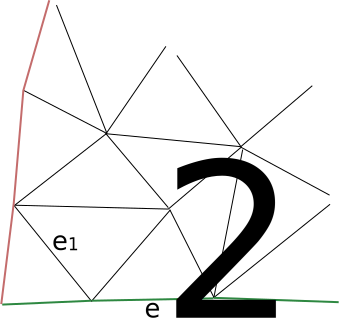
\includegraphics[width=\imagewidth]{contraction_arete_cas_1_1_avant}
	\label{fig:contraction_arete_cas_1_1_avant}
  }
  \hfill%
  \subbottom[Maillage résultant de la contraction de l'arête $e_2$.]{
	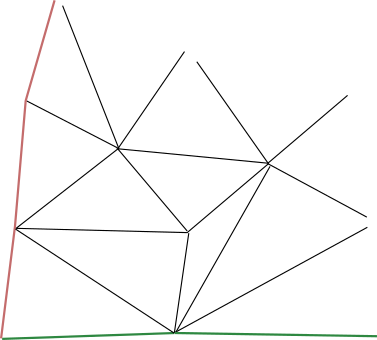
\includegraphics[width=\imagewidth]{contraction_arete_cas_1_1_apres}
	\label{fig:contraction_arete_cas_1_1_apres}
  }
  \hspace*{\fill}
  \caption{Deux cas possibles pour une arête dont les deux sommets ont un seul degré de liberté.}
  \label{fig:contraction_arete_cas_1_1}
  %
\end{figure}